\documentclass[11pt]{article}
\usepackage{makeidx}
\usepackage{multirow}
\usepackage{multicol}
\usepackage[dvipsnames,svgnames,table]{xcolor}
\usepackage{graphicx}
\usepackage{epstopdf}
\usepackage{ulem}
\usepackage{hyperref}
\usepackage{amsmath}
\usepackage{amssymb}
\author{Boy}
\title{}
\usepackage[paperwidth=595pt,paperheight=841pt,top=113pt,right=85pt,bottom=85pt,left=113pt]{geometry}

\makeatletter
	\newenvironment{indentation}[3]%
	{\par\setlength{\parindent}{#3}
	\setlength{\leftmargin}{#1}       \setlength{\rightmargin}{#2}%
	\advance\linewidth -\leftmargin       \advance\linewidth -\rightmargin%
	\advance\@totalleftmargin\leftmargin  \@setpar{{\@@par}}%
	\parshape 1\@totalleftmargin \linewidth\ignorespaces}{\par}%
\makeatother 

% new LaTeX commands


\begin{document}


\begin{center}


\textbf{{\Large ``PEMBUATAN WEBSITE PENJUALAN KOMPUTER SECARA ONLINE DI JAYA
COMPUTER KENCONG''}}
\end{center}

\begin{figure}[ht!]
  \centering
    
\includegraphics[width=5cm]{gambar/LogoUnmuh}
\end{figure}

\begin{center}
\textbf{Disusun oleh:}
\end{center}

\begin{center}
(Vani Tri Agustian)
\end{center}

\begin{center}
(1200631025)
\end{center}

\begin{center}
\textbf{JURUSAN MANAJEMEN INFORMATIKA}
\end{center}

\begin{center}
\textbf{FAKULTAS TEKNIK}
\end{center}

\begin{center}
\textbf{UNIVERSITAS MUHAMMADIYAH JEMBER}
\end{center}

\begin{center}
\textbf{2014}
\end{center}

\newpage

\begin{center}
\textbf{BAB I
\\
PENDAHULUAN}
\end{center}

\textbf{1.1. LATAR BELAKANG MASALAH}

Komputer adalah sebuah alat yang bekerja secara sistematis yang terdiri dari
elemen input, proses, dan output untuk memenuhi kebutuhan komputasi. Toko
komputer merupakan sebuah badan usaha yang menjual berbagai komponen yang
diperlukan untuk membangun sebuah komputer. Pesatnya perkembangan teknologi telah
memicu peningkatan kebutuhan masyarakat akan komputer. Teknologi kini berkembang
semakin canggih dan masyarakat berkembang menjadi lebih pandai dalam memanfaatkan
teknologi. Berbagai macam solusi teknologi dalam dunia komputer menyebabkan
masyarakat memiliki banyak pilihan untuk memilih spesifikasi komputer sesuai
kebutuhanya.

Peran toko komputer adalah menyediakan komponen yang diperlukan untuk membangun
sebuah komputer untuk memenuhi kebutuhan masyarakat akan sumber daya komputer.
Selain itu, toko komputer juga berperan sebagai konsultan bagi masyarakat yang
ingin membeli komputer namun masih awam tentang komputer.

Pesatnya perkembangan teknologi juga diikuti dengan pesatnya perkembangan
internet di masyarakat. Semakin murah dan mudahnya menggunakan internet membuat
internet menjadi semakin populer di masyarakat. Hampir semua lapisan masyarakat
telah mengenal internet sebagai layanan serba guna. Masyarakat memanfaatkan
internet untuk berbagai kebutuhan, antara lain browsing, chatting hingga jual
beli melalui secara online melalui internet. Pesatnya perkembangan internet
merupakan sebuah peluang untuk mengembangkan usaha dengan membuat website untuk
sarana promosi serta penjualan online. Transaksi jual beli secara online memiliki
banyak kelebihan yang menguntungkan bagi penjual maupun pembeli.

Keuntungan bagi pembeli, antara lain tidak perlu keluar rumah untuk membeli
barang, barang yang dibeli diantar ke rumah jadi pembeli tidak perlu
repot membawa barang serta lebih aman dari ancaman kriminalitas dan hemat waktu.

Sedangkan keuntungan bagi penjual adalah tidak memerlukan biaya besar untuk
memulai penjualan online. Banyaknya kelebihan yang dimiliki transaksi jual beli
secara online serta makin maraknya penggunaan internet menyebabkan perusahaan
besar hingga usaha kecil memiliki peluang yang sama untuk mendapatkan keuntungan
dari penjualan online melalui website.

Sehubungan dengan uraian di atas, maka penelitian ini dimaksudkan untuk
mengembangkan usaha dengan cara membuat website penjualan secara online untuk
Jaya Computer sehingga pembahasan penelitian ini dengan mengambil judul
``Pembuatan Website Penjualan Komputer Secara Online Di Jaya Computer Kencong''.

\textbf{1.2. RUMUSAN MASALAH}

Dengan latar belakang permasalahan di atas, maka rumusan yang dapat diuraikan
adalah:

\begin{itemize}
	\item Bagaimana cara membuat rancangan website untuk penjualan secara online di toko
Jaya Computer Kencong.
	\item Bagaimana agar pembuatan website penjualan komputer secara online di Jaya
Computer Kencong menjadi sarana untuk promosi, pengembangan usaha, serta sarana
penjualan yang menguntungkan.
\end{itemize}

\textbf{1.3. BATASAN MASALAH}

\begin{itemize}
	\item Sistem web hanya berjalan sebagai media penyampaian informasi seputar kegiatan
perusahaan dan penjualan produk.
	\item Cara pembayaran hanya dapat dilakukan dengan PayPal.
	\item 
Website  toko online  ini tidak terintegrasi dengan sistem jasa pengiriman.
	\item Website toko online ini tahap awal digunakan untuk pemesanan penjualan,
pencarian barang. Akan tetapi tidak membahas pengembalian barang, keamanan
website dan jaringan.
	\item Adapun data yang dibutuhkan adalah data produk, order, order\_detail,
order\_temp, kategori\_produk dan buku\_tamu.
\end{itemize}

\textbf{1.4. TUJUAN PENELITIAN}

Adapun tujuan dari penelitian ini adalah untuk membuat rancangan website sebagai sarana penjualan komputer secara online di toko Jaya Computer Kencong, agar website tersebut menjadi sarana penjualan dan promosi yang menguntungkan.

\textbf{1.5. MANFAAT PENELITIAN}

1. Manfaat bagi penulis:

\begin{itemize}
	\item •	Mengetahui dan memahami kelebihan dan keuntungan penjualan secara online melalui  internet.
	\item •	Agar setiap mahasiswa mampu membuat dan mendesain website yang digunakan sebagai sarana penjualan secara online.
	\item •	Syarat tugas Topik Khusus Pemrograman Web Lanjut oleh Triawan Adi Cahyanto, M.K
\end{itemize}

2. Manfaat bagi Jaya Computer:

\begin{enumerate}
	\item Untuk mengembangkan usaha dan jangkauan pasar.
	\item Meningkatkan penjualan dan keuntungan.
	\item Sebagai sarana penjualan dan promosi yang hemat dan menguntungkan.
\end{enumerate}

\newpage

\begin{center}
\textbf{BAB II
\\
LANDASAN TEORI}
\end{center}

\textbf{2.1. Definisi Toko}

``Toko adalah sebuah tempat tertutup yang di dalamnya terjadi kegiatan
\href{http://id.wikipedia.org/wiki/Perdagangan}{perdagangan} dengan jenis
\href{http://id.wikipedia.org/wiki/Benda}{benda} atau
\href{http://id.wikipedia.org/wiki/Barang}{barang} yang khusus, misalnya
\href{http://id.wikipedia.org/wiki/Toko\_buku}{toko buku}, toko
\href{http://id.wikipedia.org/wiki/Buah}{buah}, dan sebagainya. Secara fungsi
ekonomi, istilah "toko" sesungguhnya hampir sama dengan "kedai" atau "warung".
Akan tetapi pada perkembangan istilah, kedai dan warung cenderung bersifat
tradisional dan sederhana, dan warung umumnya dikaitkan dengan tempat penjualan
makanan dan minuman. Secara bangunan fisik, toko lebih terkesan mewah dan modern
dalam arsitektur bangunannya daripada
\href{http://id.wikipedia.org/wiki/Warung}{warung}. Toko juga lebih modern dalam
hal barang-barang yang dijual dan proses transaksinya''.
\uline{http://id.wikipedia.org/wiki/Toko.}

\textbf{2.1.1. Fungsi toko}

Fungsi penting ruang niaga saat ini adalah untuk memamerkan dan menjual barang
dagangan namun yang paling penting adalah hubungan antara pengunjung dan
\textit{display} barang dagangan serta antara pengunjung, \textit{display}, dan~
personil penjualan. (Panero, 2003 : 196)

\textbf{2.1.2. Sejarah Perkembangan Toko}

Perdagangan merupakan pendorong utaman timbulnya toko. Perdagangan itu sendiri
timbul karena beberapa hal, diantaranya yaitu:

\begin{itemize}
	\item Kebutuhan manusia yang tidak terbatas dan beraneka ragam jenisnya.
	\item Adanya perbedaan kecakapan antara manusia yang satu dengan yang lainnya.
	\item Letak geografis dimana manusia itu hidup.
	\item 

Latar belakang kemajuan pendidikan, kebudayaan, perhubungan dan bidang teknik
dan pertumbuhan penduduk. (Barata, 1995 : 19)
\end{itemize}

Perdagangan dalakukan pertama kali dengnn melikukan pertukaran barang dengan
barang (barter). Kemudian berkembang menjadi pertukaran dengan kulit binatang,
emas, perak yang dikeaal dengan sebutan mata uang logam. (Barata, 1995 : 25-26)

\textbf{2.1.3. Pengertian Promosi}

Adalah cara toko mengadakan komunikasi secara luas antara pihak toko dengan
khalayak atau masyarakat, untuk mempengaruhi, menarik minat dan menginformasikan
tentang visi, misi, tujuan, jasa layanan yang diadakan oleh toko.

\textbf{2.1.4. Business to Costumer}

Business to costumer merupakan mekanisme toko online (electronic shopping mall),
yaitu transaksi antara e-merchant dengan e-costumer.

\textbf{2.1.5. Pengertian Perancangan}

Perancangan merupakan satu cara yang sistematik untuk menentukan terlebih dahulu
tindakan yang akan diambil pada masa yang akan datang.

\textbf{2.1.6. Internet ( Interconnected Network)}

Internet adalah sebuah sistem komunikasi global yang menghubungkan komputer-komputer dan jaringan-jaringan komputer di seluruh dunia. Setiap komputer dan jaringan terhubung secara langsung maupun tidak langsung ke beberapa jalur utama yang disebut internet backbone dan dibedakan satu dengan yang lainnya menggunakan unique name yang biasa disebut dengan alamat IP 32 bit. Contoh: 202.155.4.230.

Komputer dan jaringan dengan berbagai platform yang mempunyai perbedaan dan ciri khas masing-masing(Unix, Linux, Windows, Mac, dll) bertukar informasi dengan sebuah prtokol standar yang dikenal dengan nama TCP/IP(Transmission Control Protokol/ Internet Protokol).


\textbf{2.2. Pengenalan Web}

World Wide Web (WWW) atau biasa disebut dengan web, merupakan salah satu sumber daya Internet yang berkembang pesat. Informasi web didistribusikan melalui pendekatan hypertext, yang memungkinkan suatu text pendek menjadi acuan untuk membuka dokumen yang lain. Dengan pendekatan hypertext ini seseorang dapat memperoleh informasi dengan meloncat dari suatu dokumen ke dokumen yang lain. Dokumen-dokumen yang dapat diaksespun dapat tersebar di berbagai mesin dan bahkan diberbagai negara.

Bagai jarring laba-laba, jejaring web telah membentang ke seluruh penjuru dunia. Tidak hanya terbatas pada lembaga-lembaga penelitian yang ingin mempublikasikan hasil riset, web juga banyak digunakan oleh perusahaan bisnis yang ingin mengiklankan produk atau untuk melakukan transaksi bisnisnya.

\textbf{2.2.1. Sejarah web}

Sejarah web dimulai pada bulan maret 1989 ketika Tim Berner-Lee yang bekerja di Laboratorium Fisika Partikel Eropa atau yang dikenal dengan nama CERN (Consei European pour la Recherce Nuclaire) yang berada di Genewa, swiss, mengajukan protokol (suatu tatacara untuk berkomunikasi) system distribusi informasi internet yang digunakan untuk berbagai informasi diantara fisikiawan.

Protocol inilah yang selanjutnya dikenal sebagai protocol World Wide Web dan dikembangkan oleh World Wide Web Consortium (W3C). sebagaimana diketahui, W3C adalah konsorsium dari sejumlah organisasi yang berkempentingan dalam pengembangan berbagai standar yang berkaitan dengan web.


\textbf{2.2.2. Aplikasi web}

Pada awalnya aplikasi web dibangun hanya dengan menggunakan bahasa yang disebut HTML (HyperText Markup Language) dan protocol yang digunakan dinamakan HTTP (Hypertext Transfer Protokol). Pada perkembangan berikutnya , sejumlah skrip dan objek dikembangkan untuk memperluas kemampuan HTML. Pada saat ini, banyak skrip seperti itu antara lain yaitu PHP da ASP, sedangkan contoh yang berupa objek antara lain adalah applet(java).

Aplikasi web sendiri dapat dibagi menjadi :

\begin{itemize}
	\item Web Statis
	\item Web Dinamis
\end{itemize}

Web statis dibentuk dengan menggunakan HTML saja. Kekurangan aplikasi seperti ini terletak pada keharusan untuk memelihara program secara terus menerus untuk mengikuti ssetiap perubahan yang terjadi. Kelemahan ini diatasi dengan model aplikasi web dinamis.

Dengan memperluas kemampuan HTML, yakni dengan menggunakan perangkat lunak tambahan, perubahan informasi dalam halaman-halaman Web dapat ditangani melalui perubahan data, bukan melalui perubahan program. Sebagai implementasinya, aplikasi web dapat dikoneksikan ke basis data. Dengan demikian perubahan informasi dapat dilakukan oleh operator atau yang bertanggungjawab terhadap kemutakhiran data, dan tidak menjadi tanggung jawab pemrogram atau web master.


Pengertian web yang dinamis juga terkadang diartikan sebagai halaman yang dilengkapi dengan animasi gambar, selain dapat berinteraksi dengan basis data.

Arsitektur aplikasi web :

Klien berinteraksi dengan web server, secara internal web server tadi akan berkomunikasi dengan middleware dan middleware inilah yang akan berhubungan dengan basis data (data base).

Web server

Adalah server yang melayani permintaan klien terhadap halaman web. Apache , IIS (Internet Information Server), dan Xitami merupakan contoh perangkat lunak web server.

Middleware

Middleware adalah perangkat lunak yang bekerja sama dengan web server dan berfungsi menerjemahkan kode-kode tertentu, menjalankan kode-kode tersebut, dan memungkinkan berinteraksi dengan basis data . PHP, ASP, dan Perl adalah beberapa contoh middleware.

Browser

Browser atau web browser adalah perangkat lunak di sisi klien yang digunakan untuk mengakses informasi web. Internet explorer, Netscape, dan Monzila merupakan contoh browser.

Prinsip kerja pengaksesan dokumen web yang berbasis HTML adalah seperti berikut:

\begin{enumerate}
	\item Browser meminta sebuah halaman ke suatu situs web melalui protocol HTTP.
	\item Permintaan diterima oleh web server.
	\item Web server segera mengirimkan dokumen HTML yang diminta ke klien.
	\item Browser pada klien segera menampilkan dokumen yang diterima berdasarkan kode-kode pemformat yang terdapat pada dokumen HTML.
\end{enumerate}

Dengan menggunakan pendekatan web dinamis dimungkinkan untuk membentuk aplikasi berbasis web (web-based application). Sebagai contoh, system informasi akademis berbasis web memungkinkan seseorang mahasiswa melihat informasi nilai dari matakuliah-matakuliah yang sudah diambilnya dari luar kampus (dimana saja). Selain itu, pada masa semerter baru, mahasiswa dapat memasukkan data  krs (kartu rencana studi) melalui internet.

\textbf{2.2.3.	Teknologi web}

Dari sisi teknologi yang digunakan untuk membentuk Web Dinamis, terdapat dua macam pengelompokan, yaitu:

\begin{itemize}
	\item Teknologi pada sisi klien (\textit{client-side technology})
	\item Teknologi pada sisi server (\textit{server-side technology})
\end{itemize}

\begin{itemize}
	\item Teknologi web pada sisi klien
\end{itemize}

Teknologi web pada sisi klien diimplementasikan dengan mengirimkan kode perluasan HTML atau program tersendiri dan HTML ke klien. Klienlah yang bertanggung jawab dalam melakukan proses terhadap seluruh kode yang diterima.

Kelemahan pendekatan seperti ini adalah terdapat kemungkinan bahwa browser pada klien tidak mendukung fitur kode perluasan HTML. Sebagai contoh kode VBScript yang dilekatkan pada kode HTML tidak akan berfungsi sekiranya browser yang digunakan klien tidak mendukungnya. Kelebihan teknologi pada sisi klien adalah memungkinkan penampilan yang bersifat dinamis, misalnya menampilkan jam yang terus menerus berubah ataupun untuk membuat animasi gambar yang mengikuti gerakan penunjuk mouse.

Yang termasuk dalam teknologi pada sisi klien:

\begin{itemize}
	\item Kontrol ActiveX
	\item JavaApplet
	\item Skrip sisi-klien (misalnya JavaScrpit)
\end{itemize}

\begin{itemize}
	\item Kontrol ActiveX
\end{itemize}

Adalah suatu komponen yang ditulis dengan menggunakan perangkat lunak seperti visual C++, Visual BASIC, atau Delphi. Jika komponen ini ditambahkan ke dokumen web, maka fungsi yang didukungnya akan tersaji dalam halaman web. Misalnya, kontrol ActiveX dapat digunakan untuk menampilkan grafik tiga dimensi atau bahkan untuk mengimplementasikan permainan (game) yang interaktif.

Di dalam dokumen HTML, kontrol ActiveX dilekatkan melalui tag <OBTECT>. Dalam hal ini server akan mengirimkan kode program yang melibatkan Applet dan HTML itu sendiri.

Sejauh ini ActiveX hanya berjalan di lingkungan Windows, dan hanya browser tertentu (misalnya Internet Explorer) yang dapat memprosesnya.

\begin{itemize}
	\item Java Applet
\end{itemize}

Applet adalah program yang ditulis dengan menggunakan bahasa pemrograman jave. Program ini dapat diletakkan ke halaman web, melalui tag HTML bernama <APPLET> dan dapat diproses oleh browser yang mendukung java (misalnya Internet Explorer dan Netscape). Dalam hal ini server akan mengirimkan kode applet dan HTML.

Berbeda dengan ActiveX, Applet bersifat cross-platform; artinya, dapat berjalan pada berbagai platform, asalkan platform tersebut mendukung java.


\begin{itemize}
	\item Skrip Sisi-Klien
\end{itemize}

Adalah kode-kode yang dilekatkan menjadi satu dengan kode HTML dan skrip ini diproses di klien. Dua skrip di sisi klien yang terkenal adalah JavaSkrip dan VBSkrip. JavaSkrip adalah skrip yang sangat popular dan dapat berjalan pada hampir semua browser masa kini. Adapun VBSkrip hanya berjalan di Internet Explorer.

Saat ini skrip yang disebut CSS (Cascading Style Sheets) dan dikenal dengan sebutan Dynamic HTML (DHTML) mulai banyak digunakan. Skrip ini dapat digunakan untuk memformat halaman web dengan definisi skrip ditulis terpisah ataupun menyatu dengan HTML.


\begin{itemize}
	\item Teknologi Web pada Sisi Server
\end{itemize}

Teknologi web pada sisi server memungkinkan pemrosesan kode didalam server sehingga kode yang sampai pada pemakai berbeda dengan kode asli pada server.

Keuntungan penggunaan teknologi pada sisi server adalah:


\begin{enumerate}
	\item Mengurangi lalu-lintas jaringan dengan cara menghindari percakapan bolak-balik antara klien dan server.
	\item Mengurangi waktu pemuatan kode, mengingat klien hanya mengambil kode HTML saja.
	\item Mencegah masalah ketidakkompatibelan browser.
	\item klien dapat berinteraksi dengan data yang ada pada server.
	\item Mencegah klien mengetahui rahasia kode (mengingat kode yang diberikan ke klien berbeda dengan kode asli pada server).
\end{enumerate}

Beberapa contoh teknologi yang berjalan di server adalah :

\begin{enumerate}
	\item Common Gateway Interface (CGI)
	\item Proprietary Web Server API
	\item Active Server Page (ASP)
	\item Server-Side JavaSkript
	\item Java Servlets dab JavaServer Page (JSP)
	\item PHP
\end{enumerate}

\textbf{1. Common Gateway Interface (CGI)}

Pada awalnya, technology yang umum digunakan untuk menyajikan data yang bersifat dinamis di lingkungan web adalah CGI. Pada prinsipnya CGI dapat ditulis dengan menggunakan bahasa apa aja. Namun, yang paling popular adalah Perl.

Kelemahan CGI terletak pada penciptaan proses sebanyak permintaan dari klien. Jika terjadi jumlah permintaan yang sangat banyak maka akan cendrung melumpuhkan server.

\textbf{2. Proprietary Web Server API}

Microsoft dan Netscape menciptakan API (Aplication Programming Interface) yang ditujukan untuk membuat aplikasi Web dinamis. Pustaka dari Microsoft dinamakan ISAPI (Internet Server API) dan pustaka yang dibuat oleh Netscape disebut NSAPI (Netscape Server API). Kedua API ini dimaksudkan untuk mengatasi kelemahan CGI, karena keduanya dirancang untuk menciptakan sebuah proses saja, sekalipun terdapat banyak permintaan.

\textbf{3. Active Server Page (ASP)}

ASP merupakan teknologi di sisi server yang paling banyak digunakan dilingkungan windows. Saat ini ASP juga diusahakan untuk berjalan pada platform selain windows. Teknologi lanjutan dari ASP adalah ASP.net.

\textbf{4. Server-side JavaScript}

Server-side JavaScript (SSJS) merupakan buatan Netscape yang ditujukan untuk menyaingi ASP. Dalam prakteknya, skrip ini kurang popular.

\textbf{5. Java Servlets dan JavaServer Page (JSP)}

Baik JavaServlets maupun Java Server Page menggunakan bahasa java. Oleh karena itu para pemrogram yang telah terbiasa dengan Java dapat memanfaatkan fitur Java untuk membuat program yang canggih. Sayangnya, bahasa Java meskipun tidak sesulit C tetap dianggap rumit bagi pemula. Oleh karena itu, pemakai Java Servlets dan JSP masih kalah dengan ASP atau PHP.

\textbf{6. PHP}

PHP merupakan skrip yang berjalan di server dan sangat popular dilingkungan Linux. Saat ini PHP dapat berjalan pada berbagai platform, dari UNIX hingga Windows.

\textbf{2.2.4. Database Server MySQL}

MySQL adalah suatu perangkat lunak database relasi (Relational Database Management System atau RDBMS), seperti halnya ORACLE, Postgresql, MS SQL, dan sebagainya. MySQL AB menyebut produknya sebagai database open source terpopuler di dunia. Berdasarkan riset dinyatakan bahwa bahwa di platform Web, dan baik untuk kategori open source maupun umum, MySQL adalah database yang paling banyak dipakai. Menurut perusahaan pengembangnya, MySQL telah terpasang di sekitar 3 juta komputer. Puluhan hingga ratusan ribu situs mengandalkan MySQL bekerja siang malam memompa data bagi para pengunjungnya.

\textbf{2.2.5. PayPal}

PayPal adalah salah satu alat pembayaran (Payment procesors) menggunakan internet yang terbanyak digunakan di dunia dan teraman. Pengguna internet dapat membeli barang di ebay, lisensi software original, keanggotaan situs, urusan bisnis, mengirim dan menerima donasi/sumbangan, mengirim uang ke pengguna PayPal lain di seluruh dunia dan banyak fungsi lainnya dengan mudah dan otomatis menggunakan internet, PayPal mengatasi kekurangan dalam pengiriman uang tradisional seperti Cek atau Money order yang prosesnya dapat memakan waktu PayPal seperti rekening bank, pertama kita membuat account, lalu mengisi account tersebut dengan dana dari kartu kredit atau transferan dana dari account paypal orang lain ke balance paypal kita, dan kita sudah dapat menggunakan account PayPal untuk bertransaksi Februari 2008 PayPal sudah menerima 190 negara dan 16 mata uang, pengguna PayPal Indonesia masih harus menggunakan hitungan US dollar karena rupiah belum ada di PayPal.

PayPal mempunyai cara pembayaran yang praktis, sehingga pelanggan yang akan melakukan pembayaran akan dimudahkan dalam proses transaksi.

\newpage

Berikut cara kerja dari  PayPal.

\begin{figure}[ht!]
  \centering
    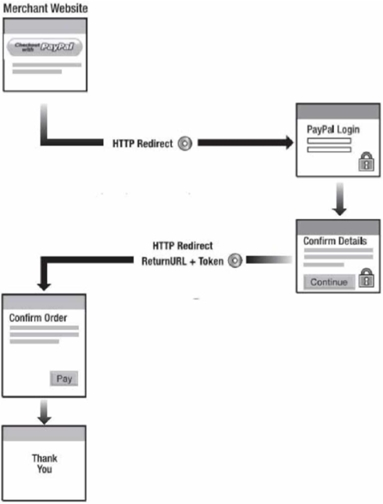
\includegraphics[width=10cm]{gambar/paypal}
    \label{paypal}
\end{figure}

\begin{center}
Gambar 1.1. Cara Kerja Pembayaran dengaa menggunaknn PayPal
\end{center}

Pertama pelanggan melakukan pemesanan di web penjualan yang menyediakan pembayaran dengan paypal. Proses selanjutnya adalah melakukan checkout, dengan melakukan checkout ini,website penjualan tersebut otomatis akan masuk Form paypal login, pelanggan yang sudah mempunyai account PayPal bisa langsung login di Paypal. Pelanggan yang sudah login maka pada halaman utama Paypal akan ada  rincian harga yang akan dibayar. Pelanggan melanjutkan pembayaran dengan melakukan intruksi yang ada di PayPal itu sendiri. Jika berhasil melakukan pembayaran maka data akan masuk pada PayPal web penjualan tersebut.

\newpage

\begin{center}
\textbf{BAB III
\\
METODE PENELITIAN}
\end{center}

\textbf{3.1. Lokasi Penelitian}

Toko Jaya Computer Kencong merupakan sebuah toko yang menjual berbagai macam
peralatan komputer  dan peralatan lainya yang berhubungan dengan komputer. Selain
menjual peralatan komputer toko Jaya Computer Kencong menyajikan jasa maintance
hardware dan penjualan software.

\textbf{3.1.1. Sejarah Toko Jaya Computer Kencong}

Toko Jaya Computer Kencong adalah perusahan yang bergerak di bidang penjualan
komputer. Perusahaan ini berdiri pada tahun 2009 yang cukup lama dan mampu
bersaing dengan toko - toko lainya, yang berada di daerah Kencong kabupaten
Jember.

\textbf{3.1.2. Visi dan Misi Toko Jaya Computer Kencong}

a. Visi Perusahaan

Kami akan lebih baik dan lebih cepat melayani pelanggan

b. Misi Perusahaan

Memanfaatkan sumber daya yang ada menjadi suatu peluang yang menarik.
Mengelola risiko secara efektif serta menjaga reputasi perusahaan.

\textbf{3.1.3. Struktur Organisasi}

Dalam suatu organisasi yang baik pada umumnya mempunyai struktur organisasi yang dapat untuk membatasi pembagian - pembagian kerja pada masing-masing bagian. Dalam hal ini strukutr organisasi merupakan dasar yang mempersatukan fungsi - fungsi perusahaan dan menetapkan hubungan yang pasti.

Adapun struktur organisasi toko Jaya Computer Kencong bisa di lihat dari gambar
di bawah.

\begin{figure}[ht!]
  \centering
    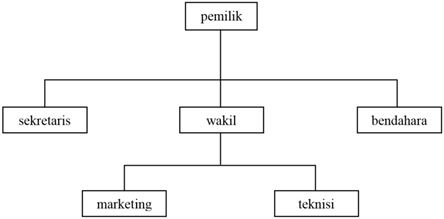
\includegraphics[width=10cm]{gambar/struktur}
    \label{struktur}
\end{figure}

\begin{center}
Gambar 1.2. Struktur Organisasi
\end{center}

\textbf{3.1.4. Deskripsi Tugas di Toko Jaya Cgmputer Kencong}

Deskripsi Tugas (Job Description ) adalah suatu rincian yang menunjukan posisi, tanggung jawab, wewenang, fungsi dan tugas yang harus dilakukan. Periode tugas perlu dibuat agar masing-masing bagian mengerti akan kedudukannya.

\newpage 

Adapun fungsi dan tugas divisi kerja yang ada di toko Jaya Computer Kencong antara lain :

1. Pemilik

Adapun tugas Pemilik yaitu :

a. Mengambil keputusan setiap kegiatan di toko Jaya Computer Kencong

b. Menerima laporan penjualan dan persediaan barang.

2. Wakil

Adapun tugas dan tanggung jawab Wakil yaitu :

a. Mengawasi kegiatan personil / pegawai toko

b. Melakukan pemesanan parang kepada sublpier jika stok barang telah habis

c. Melakukan verifikasi laporan penjualan barang, laporan persediaan barang dan
permintaan barang.

3. Sekretaris

Adapun tugas dan tanggnug jawab Sekretaris toko yaitu :

a. melakukan pembukuan hasil penjualan barang.

b. Membuat laporan penjualan, persediaan dan pembelian barang.

4. Bendahara

Adapun tugas dan tanggung jawab Bendahara toko adalah menyimpan keuangan hasil penjualan dan keuangan pembelian barang.

5. Marketing

Adapun tugas dan tanggung jawab bagian Marketing toko yaitu melayani dan menawarkan produk – produk yang di jual di toko kepada konsumen.

6. Teknisi

Adapun tugas dan tanggung jawab bagian Teknisi toko yaitu memperbaiki, merakit, instalisasi software, maintance peralatan komputer pelanggan.

\textbf{3.2. Teknik Pengumpulan Data}

Metode pengumpulan data yang penulis lakukan untuk penelitian ini yaitu menggunakan data primer dan data sekunder, berikut penjelasannya :

\textbf{3.2.1. Sumber Data Primer}

Untuk mencari dan mendapatkan data yang akurat peneliti terjun langsung kelapangan menganalisis, melihat keadaan dari sistem yang berjalan saat ini  dan memberikan evaluasi dari kinerja sistem tersebut.

1. Observasi

Observasi adalah suatu cara untuk mengumpulkan data dengan melakukan penelitian secara langsung datang ke toko Jaya Computer Kencong. Hal ini untuk mengamati dan melakukan pencatatan terhadap peristiwa yang sedang di selidiki pada objek penelitian, dan peneliti melakukan observasi dibagian penjualan dan mengamati sistem penjualan yang saat ini sedang berjalan.

2. Wawancara

Suatu teknik pengumpulan data melalui tanya jawab secara langsung antara peneliti (pengumpul data) dengan responden (sumber data), dalam hal ini wawancara dikakukan dengan responden yaitu pada pemilik toko yang berhubungan langsung dengan sistem informasi penjualan yang sedang berjalan.

\textbf{3.2.2. Sumber Data Sekunder}

Sumber data-data atau informasi lainnya yang menunjang untuk melakukan penelitian didapatkan  melalui perpustakan, internet, dan lain-lain. Studi dokumentasi yang digunakan adalah pencarian bahan-bahan atau buku-buku bacaan, karya ilmiah dan sumber-sumber bacaan lainya seperti dari internet.

\textbf{3.3. Tahapan Penelitian}

Ada beberap tahapan yang dilalui peneliti dalam mencari jawaban dari rumusan
masalah yang ditetapkan. Tahap-tahap tersebut adalah sebagai berikut :

\begin{itemize}
	\item Tahap pra lapangan, tahap ini merupakan tahap awal yang peneliti lakukan sebelum memasuki lapangan. Tahap ini meliputi membuat proposal penelitian untuk menentukan latar belakang masalah, fokus penelitian, tujuan dan manfaat penelitian dilakukan. Menyusun rancangan penelitian untuk mendesain langkah-langkah yang harus dilakukan agar penelitian bisa terlaksana seperti kapan dan dimana penelitian akan dilaksanakan, bagaimana cara mencari subyek dan informan, bagaimana pendekatan yang harus dilakukan, dan membuat guidance wawancara.
	\item Tahap pekerjaan lapangan, tahap ini adalah dimana peneliti terjun ke lapangan melakukan penelitian. Dalam hal ini, peneliti melakukan wawancara dengan subyek penelitian dan informan untuk memperoleh data guna menjawab fokus permasalahan yang telah diambil.
	\item Tahap analisis data, tahap ini dilakukan peneliti setelah seluruh data yang diperlukan telah terkumpul. Peneliti akan melakukan pemeriksaan keabsahan data. Kemudian data ini akan ditelaah secara sistematis dan diambil sebuah kesimpulan sebagai jawaban dari fokus permasalahan dalam penelitian yang telah dilakukan.
\end{itemize}

\textbf{3.3.1. Pengambilan Data}

Metode pengumpulan data adalah cara untuk memperoleh bahan-bahan yang relevan. Menurut Hadi (1990:136) agar dalam penelitian ini memperoleh data yang valid, maka metode pengumpulan data yang digunakan adalah :

a. Wawancara Mendalam

Wawancara mendalam adalah penelitian yang dilakukan dengan cara melakukan percakapan antara orang (peneliti dan informan) yang dimulai pewawancaraan antara dua orang (peneliti dengan informan) dengan tujuan khusus memperoleh keterangan yang sesuai dengan penelitian. Dan dipusatkan pada isi yang dititikberatkan pada tujuan deskripsi. Prediksi dan penjelasan sistematik mengenai penelitian tersebut. Wawancara mendalam dengan narasumber (informan) banyaknya dibatasi, dengan alasan waktu yang tersedia untuk melakukan wawancara terbatas. apabila informasi oleh peneliti masih dianggap kurang maka penelitian tersebut dilakukan di hari selanjutnya sehingga mendapatkan informasi sesuai dengan penelitian.

\textbf{3.3.2. Analisis Data}

Analisis data dalam penelitian kualitatif dilakukan dengan jalan bekerja dengan data, mengorganisasikan data berdasarkan tema, memilah-milah menjadi satuan yang dapat dikelolah, mensistensikan, menentukan dan menemukan pola, menemukan apa yang penting dan yang akan dipelajari dan memutuskan apa yang dapat dipublikasikan pada orang lain (Moleong, 2005:248).

Dalam penelitian ini peneliti mengkategorikan data-data yang relevan dengan fokus masalah yang telah peneliti tetapkan. Data mana yang dapat dikategorikan sebagai jawaban dari bagaimana cara membuat rancangan website untuk penjualan secara online di toko Jaya Computer Kencong dan bagaimana agar pembuatan website penjualan komputer secara online di Jaya Computer Kencong menjadi sarana untuk promosi, pengembangan usaha, serta sarana penjualan yang menguntungkan.

\textbf{3.3.3. Optimasi}

Teknik optimasi data yang dilakukan dalam penelitian kualitatif ini adalah melalui beberapa cara yakni :

\begin{enumerate}
	\item Perpanjangan keikutsertaan peneliti akan meningkatkan derajat kepercayaan data yang dikumpulkan. Oleh karena itu, peneliti melakukan wawancara dengan subyek maupun informan penelitian secara bertahap.
	\item Ketekunan pengamatan peneliti terhadap pembuatan website penjualan komputer secara online di Jaya Computer Kencong. Jika perpanjangan keikutsertaan penelitian menyediakan lingkup, maka menyediakan kedalaman temuan-temuan persoalan.
	\item Triangulasi data dengan melakukan perbandingan data wawancara subyek dengan data yang diperoleh dari luar sumber lainnya. Sehingga optimasi data dapat dipertanggungjawabkaN.
\end{enumerate}

\textbf{3.3.4. Analisis Hasil}

Pada tahap analisis hasil dan uji coba, peneliti akan mencoba menginputkan beberapa data dalam tabel transaksi penjualan, hal ini dilakukan  untuk menguji output yang ada di dalam website sudah sesuai dengan rumus yang telah di dapat dari jurnal. Setelah dirasa sudah memadai untuk di demokan kepada pemilik toko, maka peneliti akan mendemokan kepada pemilik toko Jaya Computer Kencong tentang bagaimana alur berjalannya website terseb

\textbf{3.4. Jadwal Penelitian}

\begin{figure}[ht!]
  \centering
    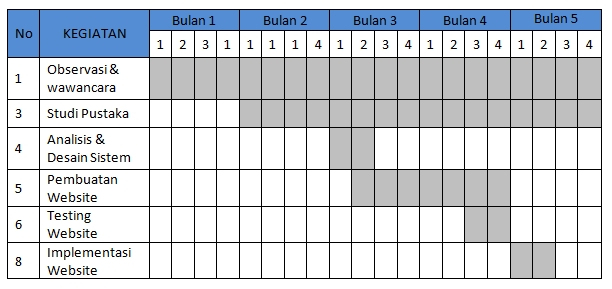
\includegraphics[width=13cm]{gambar/Jadwal}
    \label{Jadwal}
\end{figure}

\end{document}